\chapter{Benchmark Orchestration and Scheduling}
\label{ch:scheduler}

Chapters~\ref{ch:handshake} through~\ref{ch:suites} showed how to build a
single encrypted session for one cipher suite.  But to \emph{evaluate} all 72
suites we need an automated pipeline that cycles through every suite,
starts and stops proxies on both machines, collects metrics, handles failures,
and writes results to persistent storage—all without human intervention.
This chapter describes that pipeline: the \textbf{benchmark orchestration
scheduler}.

\begin{keyinsight}
The scheduler is not a real-time flight controller.  It is a lab-automation
tool that exercises every suite in sequence so that researchers can compare
them later.  Think of it as a robot lab technician that methodically runs the
same experiment 72 times, records every measurement, and neatly files the
results.
\end{keyinsight}

% ============================================================
\section{Controller--Follower Architecture}
\label{sec:sched-arch}

The benchmark involves two physical machines—Drone (Raspberry Pi~5) and GCS
(Windows laptop)—connected by a LAN cable.  One machine must be in charge of
deciding \emph{when} to switch suites and the other must comply.  We call
these roles the \textbf{controller} and the \textbf{follower}.

\begin{designdecision}
The \emph{drone} is the controller.  This may seem surprising—isn't the GCS
more powerful?  Yes, but in a real mission the drone is the constrained device
whose performance we want to measure under stress.  Making it the controller
lets us time every operation from the drone's perspective, which is the
perspective that matters for resource-constrained analysis.
\end{designdecision}

\begin{itemize}
  \item \textbf{Drone Controller} (\texttt{sdrone\_bench.py}):
        Decides when to advance to the next suite, starts its own proxy,
        reads handshake metrics, collects MAVLink and system metrics,
        and writes all results to disk.
  \item \textbf{GCS Follower} (\texttt{sgcs\_bench.py}):
        Listens for commands from the drone on a TCP control channel,
        starts/stops its own proxy on demand, collects GCS-side
        validation metrics, and returns them to the drone upon request.
\end{itemize}

Figure~\ref{fig:sched-roles} shows the high-level interaction.

\begin{figure}[htbp]
\centering
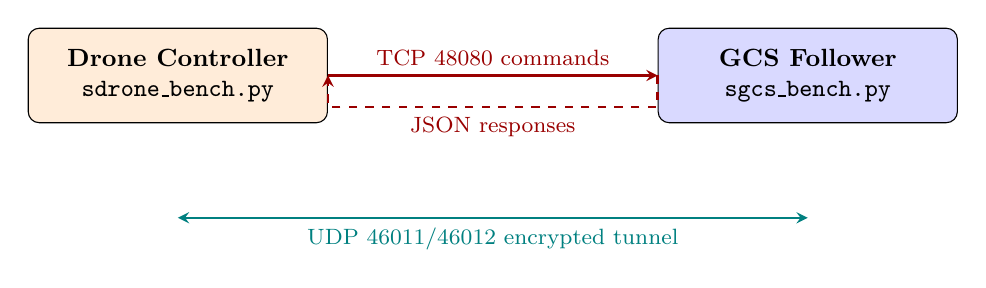
\begin{tikzpicture}[
    box/.style={draw, rounded corners, minimum width=3.8cm,
                minimum height=1.2cm, align=center, font=\small},
    arr/.style={->, >=stealth, thick}
  ]
  % Drone
  \node[box, fill=orange!15] (drone) at (0,0) {%
    \textbf{Drone Controller}\\
    \texttt{sdrone\_bench.py}};
  % GCS
  \node[box, fill=blue!15] (gcs) at (8,0) {%
    \textbf{GCS Follower}\\
    \texttt{sgcs\_bench.py}};
  % Control channel
  \draw[arr, color=red!60!black] (drone.east) -- node[above, font=\footnotesize]
    {TCP 48080 commands} (gcs.west);
  \draw[arr, color=red!60!black, dashed] (gcs.west) -- ++(0,-0.4)
    -| node[below, font=\footnotesize, pos=0.25]
    {JSON responses} (drone.east |- 0,-0.4) -- (drone.east);
  % Crypto tunnel
  \draw[arr, color=teal, <->] ([yshift=-1.2cm]drone.south) --
    node[below, font=\footnotesize] {UDP 46011/46012 encrypted tunnel}
    ([yshift=-1.2cm]gcs.south);
\end{tikzpicture}
\caption{Controller--follower architecture.  The drone sends commands over
a plaintext TCP control channel; the encrypted tunnel carries MAVLink data.}
\label{fig:sched-roles}
\end{figure}

% ============================================================
\section{The TCP Control Channel}
\label{sec:sched-tcp}

The control channel is a simple JSON-over-TCP protocol.  The drone opens a
fresh TCP connection to \texttt{GCS\_CONTROL\_HOST:48080} for every command,
sends a single JSON object terminated by a newline, reads the response, and
closes the socket.  Table~\ref{tab:sched-cmds} lists the supported commands.

\begin{table}[htbp]
\centering
\caption{TCP control channel commands}
\label{tab:sched-cmds}
\begin{tabular}{@{}l l p{6.5cm}@{}}
\toprule
\textbf{Command} & \textbf{Direction} & \textbf{Description} \\
\midrule
\texttt{ping}           & D $\to$ G & Liveness check; GCS responds ``pong'' \\
\texttt{get\_info}      & D $\to$ G & Returns GCS hostname, IP, kernel, Python version \\
\texttt{chronos\_sync}  & D $\to$ G & Clock synchronisation (NTP-lite 3-way handshake) \\
\texttt{start\_proxy}   & D $\to$ G & Start GCS-side proxy for a given suite and run ID \\
\texttt{prepare\_rekey} & D $\to$ G & Stop GCS proxy in preparation for suite switch \\
\texttt{start\_traffic} & D $\to$ G & Start synthetic UDP traffic (disabled in MAVProxy mode) \\
\texttt{stop\_suite}    & D $\to$ G & Stop current suite and return GCS-side metrics \\
\texttt{shutdown}       & D $\to$ G & Graceful server shutdown \\
\bottomrule
\end{tabular}
\end{table}

\begin{analogy}
Think of the control channel as a walkie-talkie between a pit crew chief
(drone) and the garage mechanic (GCS).  The chief says ``install suite~\#17,''
the mechanic does the work and radios back ``done.''  The actual race
(encrypted tunnel) happens on a separate track.
\end{analogy}

The \texttt{send\_gcs\_command} function on the drone side implements the
protocol:
\begin{lstlisting}[style=python, caption={Sending a command to GCS (simplified)}]
def send_gcs_command(cmd, **kwargs):
    payload = {"cmd": cmd, **kwargs}
    sock = socket.create_connection(
        (GCS_CONTROL_HOST, GCS_CONTROL_PORT),
        timeout=max(90, REKEY_HANDSHAKE_TIMEOUT + 15)
    )
    sock.sendall(json.dumps(payload).encode() + b"\n")
    data = sock.recv(65536)
    sock.close()
    return json.loads(data)
\end{lstlisting}

\subsection{Clock Synchronisation: Operation Chronos}

Before any benchmark begins, the drone and GCS must agree on a shared time
reference.  The module \texttt{core/clock\_sync.py} implements a three-way
NTP-lite handshake:

\begin{enumerate}
  \item \textbf{T1}: Drone records its wall-clock time and sends it to GCS.
  \item \textbf{T2}: GCS records the arrival time.
  \item \textbf{T3}: GCS records the departure time and responds with
        $(T_1, T_2, T_3)$.
  \item \textbf{T4}: Drone records the response arrival time.
\end{enumerate}

The clock offset (GCS~$-$~Drone) is:

\[
  \text{offset} = \frac{(T_2 - T_1) + (T_3 - T_4)}{2}
\]

The drone re-synchronises periodically—every 10~suites or every 1200~seconds,
whichever comes first—to bound cumulative drift.

\begin{securitynote}
The clock sync channel is \emph{unauthenticated} (plaintext TCP).  An active
attacker could inject false timestamps and skew the offset, making the drone
believe suite intervals are shorter or longer than they really are.  This is
acceptable in a lab setting but would need HMAC protection in a production
deployment.
\end{securitynote}

% ============================================================
\section{Benchmark Modes}
\label{sec:sched-modes}

The scheduler supports two benchmark modes, resolved by a deterministic
priority chain: CLI argument $>$ environment variable \texttt{BENCHMARK\_MODE}
$>$ default.

\begin{description}
  \item[MAVPROXY] (default):
    A physical flight controller is connected via serial, and a real
    \texttt{MAVProxy} process forwards MAVLink messages through the
    encrypted tunnel.  This mode captures genuine telemetry latency,
    jitter, and message integrity.  Synthetic traffic generation is
    \emph{disabled}.
  \item[SYNTHETIC]:
    No flight controller is present.  The scheduler generates UDP
    traffic at a configurable rate to simulate payload.  Useful for
    pure cryptographic benchmarking without hardware dependencies.
\end{description}

Both modes share the same suite-cycling logic; only the data-plane source
differs.

% ============================================================
\section{The BenchmarkPolicy}
\label{sec:sched-policy}

The \texttt{BenchmarkPolicy} class (in \texttt{sscheduler/benchmark\_policy.py})
is the decision engine that answers one question: \emph{``Should we stay on
the current suite or advance?''}

\subsection{Data Structures}

\begin{description}
  \item[\texttt{BenchmarkAction}] An enum with three values:
    \texttt{HOLD} (stay on current suite), \texttt{NEXT\_SUITE} (advance to
    the next one), and \texttt{COMPLETE} (all suites tested).

  \item[\texttt{SuiteMetrics}] A dataclass capturing every measurement for
    a single suite: handshake timing, KEM/SIG primitive breakdowns, artifact
    sizes, power, energy, throughput, latency, and a success flag.

  \item[\texttt{BenchmarkOutput}] The return value of \texttt{evaluate()}.
    Contains the proposed action, the target suite, progress percentage,
    elapsed time, and human-readable reasons.
\end{description}

\subsection{Two-Phase Commit Protocol}
\label{sec:sched-2phase}

A critical design pattern is the \textbf{two-phase commit} between
\texttt{evaluate()} and \texttt{confirm\_advance()}.

\begin{keyinsight}
\texttt{evaluate()} is a \emph{pure query}—it examines the current state and
\emph{proposes} an action (HOLD, NEXT\_SUITE, or COMPLETE) without modifying
any state.  \texttt{confirm\_advance()} is the \emph{commit}—it advances the
index, starts metrics for the next suite, and (on COMPLETE) saves results.
The caller \emph{must} call \texttt{confirm\_advance()} exactly once per
accepted proposal.
\end{keyinsight}

Why this separation?  Because the caller may need to perform work between the
decision and the commit:

\begin{enumerate}
  \item \texttt{evaluate(now)} $\to$ \texttt{NEXT\_SUITE}
  \item Caller collects GCS metrics for the current suite.
  \item Caller finalises the current suite's metrics
        (\texttt{finalize\_suite\_metrics}).
  \item Caller calls \texttt{confirm\_advance(now)} to commit the advance.
  \item Caller stops the old proxy and starts the new one.
\end{enumerate}

\begin{implementationnote}
The ordering in step~2--4 is \textbf{critical}: metrics must be finalised
\emph{before} the index advances, because \texttt{confirm\_advance()} calls
\texttt{\_start\_suite\_metrics()} for the \emph{next} suite.  If the order
were reversed, the finalised metrics would belong to the wrong suite.
\end{implementationnote}

\subsection{Suite Cycling}

The policy builds an ordered list of suites at initialisation time:

\begin{enumerate}
  \item Start with all suites from the registry (\texttt{list\_suites()}).
  \item Optionally filter by AEAD (e.g.\ \texttt{--filter-aead aesgcm}).
  \item Sort by (NIST level, KEM name, SIG name) for reproducible ordering.
\end{enumerate}

Each suite runs for a configurable interval (default: 110~seconds).  When
\texttt{evaluate()} detects that the elapsed time on the current suite exceeds
the interval, it proposes \texttt{NEXT\_SUITE}.  When the last suite's
interval elapses, it proposes \texttt{COMPLETE}.

\subsection{Metrics Collection per Suite}

For every suite the policy tracks:

\begin{table}[htbp]
\centering
\caption{SuiteMetrics fields collected by BenchmarkPolicy}
\label{tab:sched-metrics}
\begin{tabular}{@{}l l l@{}}
\toprule
\textbf{Field} & \textbf{Type} & \textbf{Source} \\
\midrule
\texttt{handshake\_ms}     & \texttt{float} & Proxy status file \\
\texttt{kem\_keygen\_ms}   & \texttt{float} & Handshake metrics \\
\texttt{kem\_encaps\_ms}   & \texttt{float} & Handshake metrics \\
\texttt{kem\_decaps\_ms}   & \texttt{float} & Handshake metrics \\
\texttt{sig\_sign\_ms}     & \texttt{float} & Handshake metrics \\
\texttt{sig\_verify\_ms}   & \texttt{float} & Handshake metrics \\
\texttt{pub\_key\_size\_bytes}     & \texttt{int} & Handshake metrics \\
\texttt{ciphertext\_size\_bytes}   & \texttt{int} & Handshake metrics \\
\texttt{sig\_size\_bytes}          & \texttt{int} & Handshake metrics \\
\texttt{power\_w}           & \texttt{float} & Power monitor \\
\texttt{energy\_mj}         & \texttt{float} & Computed \\
\texttt{throughput\_mbps}   & \texttt{float} & Data plane counters \\
\texttt{latency\_ms}        & \texttt{float} & MAVLink timing \\
\texttt{success}             & \texttt{bool} & Handshake outcome \\
\bottomrule
\end{tabular}
\end{table}

\subsection{Result Persistence}

When the benchmark completes, \texttt{\_save\_results()} writes two files:

\begin{itemize}
  \item A \textbf{JSON} file containing all suite metrics, suite identifiers,
        run metadata, and AEAD filter settings.
  \item A \textbf{CSV} file with one row per suite, suitable for import into
        spreadsheet or data-analysis tools.
\end{itemize}

Both files are timestamped with the run ID
(\texttt{benchmark\_results\_YYYYMMDD\_HHMMSS.json}).

% ============================================================
\section{The Drone Benchmark Scheduler}
\label{sec:sched-drone}

The \texttt{BenchmarkScheduler} class in \texttt{sdrone\_bench.py} is the main
entry point on the drone side.  It orchestrates the full lifecycle:

\subsection{Initialisation}

\begin{enumerate}
  \item Parse CLI arguments: \texttt{--mav-master}, \texttt{--interval},
        \texttt{--filter-aead}, \texttt{--max-suites}, \texttt{--dry-run},
        \texttt{--gcs-host}, \texttt{--mode}.
  \item Resolve benchmark mode (MAVPROXY or SYNTHETIC).
  \item Create a \texttt{DroneProxyManager} (wraps \texttt{ManagedProcess}).
  \item Create a \texttt{BenchmarkPolicy} with the chosen interval and
        AEAD filter.
  \item Create a run-specific log directory:
        \texttt{logs/benchmarks/live\_run\_YYYYMMDD\_HHMMSS/}.
  \item Initialise the \texttt{MetricsAggregator} (comprehensive 18-category
        metrics) and the \texttt{RobustLogger} (aggressive append-mode
        JSONL logging).
\end{enumerate}

\subsection{The Main Loop}
\label{sec:sched-mainloop}

Figure~\ref{fig:sched-loop} shows the lifecycle of a single suite within the
main loop.

\begin{figure}[htbp]
\centering
\begin{tikzpicture}[
    node distance=0.65cm,
    block/.style={draw, rounded corners, minimum width=4.5cm,
                  minimum height=0.65cm, font=\footnotesize, align=center},
    decision/.style={draw, diamond, aspect=2.5, font=\footnotesize,
                     inner sep=1pt, align=center},
    arr/.style={->, >=stealth, thick}
  ]
  \node[block, fill=yellow!15] (wait) {Wait for GCS (\texttt{ping})};
  \node[block, fill=green!15, below=of wait] (sync) {Clock sync (Chronos)};
  \node[block, fill=blue!15, below=of sync] (mav) {Start MAVProxy};
  \node[block, fill=orange!15, below=of mav] (activate)
    {Activate suite $i$\\(GCS + drone proxies)};
  \node[decision, below=of activate] (hs) {Handshake\\OK?};
  \node[block, fill=green!10, below left=0.8cm and -0.8cm of hs] (run)
    {Run for interval\\(collect metrics)};
  \node[block, fill=red!10, below right=0.8cm and -0.8cm of hs] (fail)
    {Mark failed\\finalise metrics};
  \node[decision, below=1.0cm of run] (eval) {evaluate()};
  \node[block, fill=teal!15, below left=0.8cm and -0.8cm of eval] (next)
    {Collect GCS metrics\\finalise \& advance};
  \node[block, fill=purple!15, below right=0.8cm and -0.8cm of eval] (done)
    {Save results\\shutdown};

  \draw[arr] (wait) -- (sync);
  \draw[arr] (sync) -- (mav);
  \draw[arr] (mav) -- (activate);
  \draw[arr] (activate) -- (hs);
  \draw[arr] (hs) -- node[left, font=\scriptsize] {Yes} (run);
  \draw[arr] (hs) -- node[right, font=\scriptsize] {No} (fail);
  \draw[arr] (run) -- (eval);
  \draw[arr] (fail.south) |- ([yshift=-0.3cm]eval.east) -- (eval);
  \draw[arr] (eval) -- node[left, font=\scriptsize] {NEXT} (next);
  \draw[arr] (eval) -- node[right, font=\scriptsize] {COMPLETE} (done);
  \draw[arr] (next.west) -- ++(-1.5,0) |- (activate.west);
\end{tikzpicture}
\caption{Lifecycle of the benchmark main loop.  Each suite goes through
activation, handshake, metric collection, and policy evaluation.}
\label{fig:sched-loop}
\end{figure}

The \texttt{\_run\_loop()} method implements this cycle:

\begin{enumerate}
  \item Call \texttt{\_activate\_suite(suite\_name)}, which:
    \begin{itemize}
      \item Checks whether a clock re-sync is needed.
      \item Sends \texttt{start\_proxy} to GCS.
      \item Starts the drone-side proxy via \texttt{DroneProxyManager}.
      \item Waits up to 45~seconds for handshake completion (to accommodate
            Classic McEliece's large key operations).
      \item Records handshake metrics in the policy and aggregator.
    \end{itemize}

  \item Enter a polling loop that repeatedly calls
        \texttt{policy.evaluate(time.monotonic())}:
    \begin{description}
      \item[HOLD] Sleep for the remaining interval fraction
            (capped at 1~second to avoid overshooting).
      \item[NEXT\_SUITE] Collect GCS metrics, finalise the current suite,
            call \texttt{confirm\_advance()}, stop the old proxy, and
            start the new one.
      \item[COMPLETE] Same as NEXT\_SUITE, but then exit the loop.
    \end{description}

  \item Before advancing, check \texttt{\_ready\_to\_advance()}, which
        verifies that:
    \begin{itemize}
      \item MAVProxy is still alive (in MAVPROXY mode).
      \item The GCS control channel is responsive.
      \item MAVLink messages have been received.
      \item Data-plane counters are non-zero.
    \end{itemize}
    If not ready, extend the suite by up to \texttt{interval~+~10}
    seconds (the ``grace period'').
\end{enumerate}

\begin{implementationnote}
The policy always uses \texttt{time.monotonic()} rather than
\texttt{synced\_time()}.  This prevents time-domain mixing: synced time
returns a wall-clock value ($\sim 1.7 \times 10^{9}$), which would make
elapsed-time calculations meaningless when mixed with monotonic timestamps
that start near zero.
\end{implementationnote}

\subsection{The DroneProxyManager}

This helper class wraps the drone proxy subprocess:

\begin{itemize}
  \item \textbf{start(suite\_name)}: Looks up the suite, locates the
        GCS public key in \texttt{secrets/matrix/\{suite\}/gcs\_signing.pub},
        constructs the CLI command, and launches it via \texttt{ManagedProcess}
        with output redirected to a timestamped log file.
  \item \textbf{stop()}: Terminates the managed process, closes the log
        file handle (to prevent file-descriptor leaks), and resets state.
  \item \textbf{is\_running()}: Delegates to \texttt{ManagedProcess.is\_running()}.
\end{itemize}

\subsection{Handshake Status Reader}

After starting the drone proxy, the scheduler polls a JSON status file
(\texttt{drone\_status.json}) for up to 45~seconds.  The proxy writes this
file immediately after handshake completion with one of two statuses:

\begin{itemize}
  \item \texttt{"handshake\_ok"}: Written right after handshake success,
        containing the full handshake metrics.
  \item \texttt{"running"}: Written during periodic status updates.
        Both are accepted as proof of a successful handshake.
\end{itemize}

% ============================================================
\section{The GCS Benchmark Server}
\label{sec:sched-gcs}

The GCS side runs a \texttt{GcsBenchmarkServer} (in \texttt{sgcs\_bench.py})
that listens on TCP~48080 for drone commands.  It is entirely
\emph{reactive}—it never initiates a suite switch on its own.

\subsection{Component Stack}

\begin{table}[htbp]
\centering
\caption{GCS server internal components}
\label{tab:sched-gcs-components}
\begin{tabular}{@{}l p{7.5cm}@{}}
\toprule
\textbf{Component} & \textbf{Responsibility} \\
\midrule
\texttt{GcsProxyManager}         & Starts/stops GCS proxy subprocesses \\
\texttt{GcsMavProxyManager}      & Manages MAVProxy with optional GUI (--map --console) \\
\texttt{MavLinkMetricsCollector} & Sniffs MAVLink on UDP~14552 for validation \\
\texttt{GcsSystemMetricsCollector} & Samples CPU, memory, temperature at 0.5\,Hz \\
\texttt{MetricsAggregator}       & 18-category comprehensive metrics (GCS side) \\
\texttt{ClockSync}               & Server side of NTP-lite handshake \\
\texttt{RobustLogger}            & Aggressive append-mode JSONL logging \\
\bottomrule
\end{tabular}
\end{table}

\subsection{Command Handling}

Each incoming TCP connection is handled in a single thread.  The server reads
one JSON command, dispatches to the appropriate handler, and returns a JSON
response.  The most important handlers are:

\begin{description}
  \item[\texttt{start\_proxy}] Accepts a suite name and an optional
    \texttt{run\_id}.  If the drone's run ID differs from the current one,
    the server updates its log directory and reinitialises its
    \texttt{MetricsAggregator} and \texttt{RobustLogger} to write to the
    matching folder.  It then starts the GCS proxy, resets the MAVLink
    validation counters, and starts system metrics sampling.

  \item[\texttt{stop\_suite}] Stops traffic, collects MAVLink validation
    metrics (message count + sequence gap count), GCS system metrics,
    and proxy status.  Packages everything into a JSON response that the
    drone merges into its comprehensive metrics.  Also writes to a local
    JSONL log with fsync and retry (up to~3 attempts).

  \item[\texttt{chronos\_sync}] Delegates to
    \texttt{ClockSync.server\_handle\_sync()}, which records $T_2$ and $T_3$
    and returns them along with the echoed $T_1$.
\end{description}

\subsection{Consistent Log Directories}

Both machines must write to the same logical run folder.  The drone is the
authority on the \texttt{run\_id} (it is generated from the drone's UTC
timestamp at startup).  When the GCS receives a \texttt{start\_proxy} command
with a \texttt{run\_id} it hasn't seen before, it calls
\texttt{\_update\_run\_id()}, which:

\begin{enumerate}
  \item Creates a new directory \texttt{logs/benchmarks/live\_run\_\{run\_id\}/}.
  \item Stops and replaces the old \texttt{GcsProxyManager}.
  \item Reinitialises the \texttt{MetricsAggregator} and \texttt{RobustLogger}
        with the new run ID.
\end{enumerate}

% ============================================================
\section{Scheduling Policies}
\label{sec:sched-policies}

The codebase contains several scheduling policies beyond the benchmark policy.
These are defined in \texttt{sscheduler/policy.py} and are used by the
production (non-benchmark) scheduler.

\subsection{TelemetryAwarePolicyV2}

This is the \emph{safety-critical} policy intended for real flight operations.
It consumes both GCS telemetry (link quality) and local drone telemetry
(battery, temperature) to make rekey and suite-switch decisions.

\begin{table}[htbp]
\centering
\caption{Decision hierarchy of TelemetryAwarePolicyV2}
\label{tab:sched-telemv2}
\begin{tabular}{@{}c l p{5.5cm} l@{}}
\toprule
\textbf{Priority} & \textbf{Gate} & \textbf{Condition} & \textbf{Action} \\
\midrule
1 & Safety gate     & Telemetry stale ($> 2\,$s) & HOLD \\
2 & Emergency       & Battery critical or temp critical & DOWNGRADE to tier~0 \\
3 & Blackout        & $>3$ blackouts within 30\,s of switch & DOWNGRADE + blacklist \\
4 & Cooldown        & Still in cooldown window & HOLD \\
5 & Link degradation & Gap P95 $> 1\,$s or PPS $< 5$ (with hysteresis) & DOWNGRADE \\
6 & Stress          & Temp rising or battery falling fast & DOWNGRADE \\
7 & Proactive rekey & Stable $> 60\,$s and under rate limit & REKEY \\
8 & Upgrade         & Disarmed, stable, no stress (30\,s hysteresis) & UPGRADE \\
9 & Nominal         & None of the above & HOLD \\
\bottomrule
\end{tabular}
\end{table}

\subsubsection{Suite Tier Mapping}

The policy maps each suite to a numeric tier that encodes its computational
weight:

\[
\text{tier} = \underbrace{\text{level\_tier}}_{\substack{0 = L1 \\ 10 = L3 \\ 20 = L5}}
+ \underbrace{\text{kem\_tier}}_{\substack{0 = \text{ML-KEM} \\ 3 = \text{HQC} \\ 5 = \text{McEliece}}}
+ \underbrace{\text{aead\_tier}}_{\substack{0 = \text{AES-GCM} \\ 1 = \text{ChaCha20} \\ 2 = \text{ASCON}}}
\]

Downgrade moves to a lower tier (lighter); upgrade moves to a higher tier
(heavier).

\subsubsection{Hysteresis}

To avoid oscillation (rapidly switching back and forth), the policy requires
that a condition persists for a configurable duration before acting:

\begin{itemize}
  \item \textbf{Downgrade hysteresis}: 5~seconds (link degradation or stress
        must persist for 5~seconds before triggering a downgrade).
  \item \textbf{Upgrade hysteresis}: 30~seconds (stable conditions must
        persist for 30~seconds before allowing an upgrade).
\end{itemize}

\subsubsection{Blacklisting}

If a suite causes link failure shortly after activation ($< 30\,$s), the
policy \emph{blacklists} it for a configurable TTL (default: 1800~seconds =
30~minutes).  Blacklisted suites are skipped during downgrade/upgrade
searches.

\subsubsection{Rekey Rate Limiting}

Rekeys are limited by a sliding window: at most $N$ successful rekeys within
$W$ seconds (default: 5 per 300~seconds).  Importantly, rekeys are only
\emph{recorded} after successful execution (via \texttt{record\_rekey()}),
not when proposed—this prevents failed rekey attempts from consuming the
quota.

\subsection{Simple Policies}

\begin{description}
  \item[\texttt{LinearLoopPolicy}] Deterministic round-robin through a given
    suite list.  Advances on every call to \texttt{next\_suite()}.
    Configurable duration per suite.

  \item[\texttt{RandomPolicy}] Selects a random suite from the pool on every
    call.  Uses its own \texttt{random.Random} instance for reproducibility.

  \item[\texttt{ManualOverridePolicy}] Normally round-robin, but accepts an
    external override via \texttt{set\_override(suite\_name)}.  When set, all
    calls to \texttt{next\_suite()} return the overridden suite.

  \item[\texttt{DeterministicClockPolicy}] Uses synchronised time (Chronos)
    to compute the suite index deterministically:
    $\text{index} = \lfloor \text{synced\_time} / \text{interval} \rfloor
    \mod |\text{suites}|$.
    Both machines independently compute the same suite without coordination.
\end{description}

% ============================================================
\section{Subprocess Management}
\label{sec:sched-process}

Both the drone and GCS start proxy and MAVProxy instances as child processes.
The \texttt{ManagedProcess} class (in \texttt{core/process.py}) provides
cross-platform process management:

\begin{itemize}
  \item \textbf{Windows}: Creates a Win32 Job Object and assigns the child
        process to it.  When the parent dies, the Job Object is closed and
        all child processes are terminated automatically.
  \item \textbf{Linux}: Sets \texttt{PR\_SET\_PDEATHSIG} via
        \texttt{ctypes.CDLL('libc.so.6')} so that the child receives
        \texttt{SIGTERM} when its parent exits.
  \item \textbf{Graceful stop}: \texttt{stop()} sends \texttt{SIGTERM}
        (or \texttt{TerminateProcess} on Windows), waits up to a timeout,
        then escalates to \texttt{SIGKILL}.
\end{itemize}

\begin{securitynote}
Without \texttt{ManagedProcess}, a crash in the scheduler would leave orphaned
proxy processes running—potentially with stale keys, consuming resources, and
occupying ports.  The Job Object / PDEATHSIG mechanism ensures that a
scheduler crash always cleans up its children.
\end{securitynote}

% ============================================================
\section{End-to-End Benchmark Flow}
\label{sec:sched-e2e}

Putting it all together, here is the complete sequence for a full benchmark
run with, say, 24~suites (filtered to AES-GCM only):

\begin{enumerate}
  \item \textbf{User starts GCS server}:
        \texttt{python -m sscheduler.sgcs\_bench --no-gui}
  \item \textbf{User starts drone scheduler}:
        \texttt{python -m sscheduler.sdrone\_bench --interval 110
        --filter-aead aesgcm}
  \item Drone resolves mode to MAVPROXY.
  \item Drone creates \texttt{BenchmarkPolicy} with 24~suites, 110\,s interval.
  \item Drone pings GCS \textrightarrow{} ``pong.''
  \item Drone performs clock sync \textrightarrow{} offset recorded.
  \item Drone starts MAVProxy.
  \item \textbf{For each suite $i = 0 \ldots 23$}:
    \begin{enumerate}
      \item Drone sends \texttt{start\_proxy(suite=\ldots, run\_id=\ldots)}
            to GCS.
      \item GCS starts its proxy subprocess.
      \item Drone starts its proxy subprocess.
      \item Both proxies perform the PQC handshake (Chapter~\ref{ch:handshake}).
      \item Drone reads handshake metrics from status file.
      \item Encrypted MAVLink flows for $\sim 110\,$seconds.
      \item \texttt{policy.evaluate()} returns \texttt{NEXT\_SUITE}
            (or \texttt{COMPLETE}).
      \item Drone sends \texttt{stop\_suite} to GCS, receives GCS metrics.
      \item Drone calls \texttt{finalize\_suite\_metrics()} then
            \texttt{confirm\_advance()}.
      \item Both proxies are stopped; next suite begins.
    \end{enumerate}
  \item Drone saves final summary JSON.
  \item Drone and GCS both shut down cleanly.
\end{enumerate}

For 24 suites at 110~seconds each, the entire run takes approximately
$24 \times 110 = 2{,}640$ seconds $\approx$ 44~minutes.  For all 72~suites:
$72 \times 110 = 7{,}920$ seconds $\approx$ 2~hours 12~minutes.

% ============================================================
\section{Error Handling and Resilience}
\label{sec:sched-errors}

\begin{itemize}
  \item \textbf{Handshake timeout}: If the proxy handshake does not complete
        within 45~seconds, the suite is marked as failed
        (\texttt{success=False}) and metrics are finalised with the error
        reason.  The benchmark continues to the next suite.
  \item \textbf{GCS unreachable}: If \texttt{send\_gcs\_command} times out,
        the result contains \texttt{status: error}.  The scheduler logs the
        failure and may retry or skip.
  \item \textbf{MAVProxy crash}: In MAVPROXY mode, if \texttt{mavproxy\_proc}
        is no longer running, the scheduler aborts with
        \texttt{shutdown\_reason=``error: mavproxy\_died''}.
  \item \textbf{Ctrl-C}: The signal handler calls \texttt{cleanup\_environment},
        which stops all managed processes.  An \texttt{atexit} handler
        provides a second safety net.
  \item \textbf{Re-entrancy guard}: The \texttt{\_cleanup()} method uses a
        boolean flag (\texttt{\_cleanup\_done}) to prevent double-cleanup if
        called from both the signal handler and atexit.
\end{itemize}

% ============================================================
\section{Chapter Summary}

\begin{itemize}
  \item The benchmark scheduler follows a \textbf{controller--follower}
        architecture: the drone decides, the GCS obeys.
  \item A \textbf{TCP JSON control channel} on port~48080 carries
        commands and metric responses between the two machines.
  \item \textbf{Clock synchronisation} (Operation Chronos) uses a 3-way
        NTP-lite handshake to bound timing drift.
  \item \textbf{BenchmarkPolicy} implements a two-phase
        evaluate/confirm\_advance protocol that cleanly separates
        decision-making from state mutation.
  \item \textbf{TelemetryAwarePolicyV2} is the production policy with
        9-level priority, hysteresis, blacklisting, and rate limiting.
  \item \textbf{ManagedProcess} ensures cross-platform subprocess cleanup
        via Win32 Job Objects and Linux PDEATHSIG.
  \item A full 72-suite benchmark runs in approximately 2~hours 12~minutes
        with the default 110-second interval.
\end{itemize}
